\infolevone{
\section{The Solid Target Ladder}

%The scattering chamber has two target ladders, a cryogenic target ladder and a solid target ladder. 
The solid target ladder is hung directly below the cryotarget ladder,
forming a single vertical column of cryogenic and solid targets. The
solid targets are typically conductively cooled and rely on a good
thermal connection to the cryotarget ladder which provides a 20 K
thermal reservoir. A single vertical motion system with a 24 inch
stroke is used to select which target is placed on the beam axis.

Like for the LH2 target, target motion is performed by the target
operator using the main target control GUI in the Hall C counting
room. He/she must coordinate this target motion through the MCC, to
insure the target motion is masked during the motion, and unmasked
after the target has moved. The target operator should always make
sure that the beam current and raster size for the target on the beam
axis is within safe limits, as determined in advance and posted in the
operational restrictions (see below). A couple different views of the
solid target ladder are shown in \ref{fig:SolidTgtsCAD}.

\begin{figure}[!htb]
%\vspace*{-1.8cm}
\begin{center}
%\hspace*{-3.5cm}
%\includegraphics[width =0.95\textwidth,angle=-90]{Pics/QWEAK-tgt-schematic.pdf}
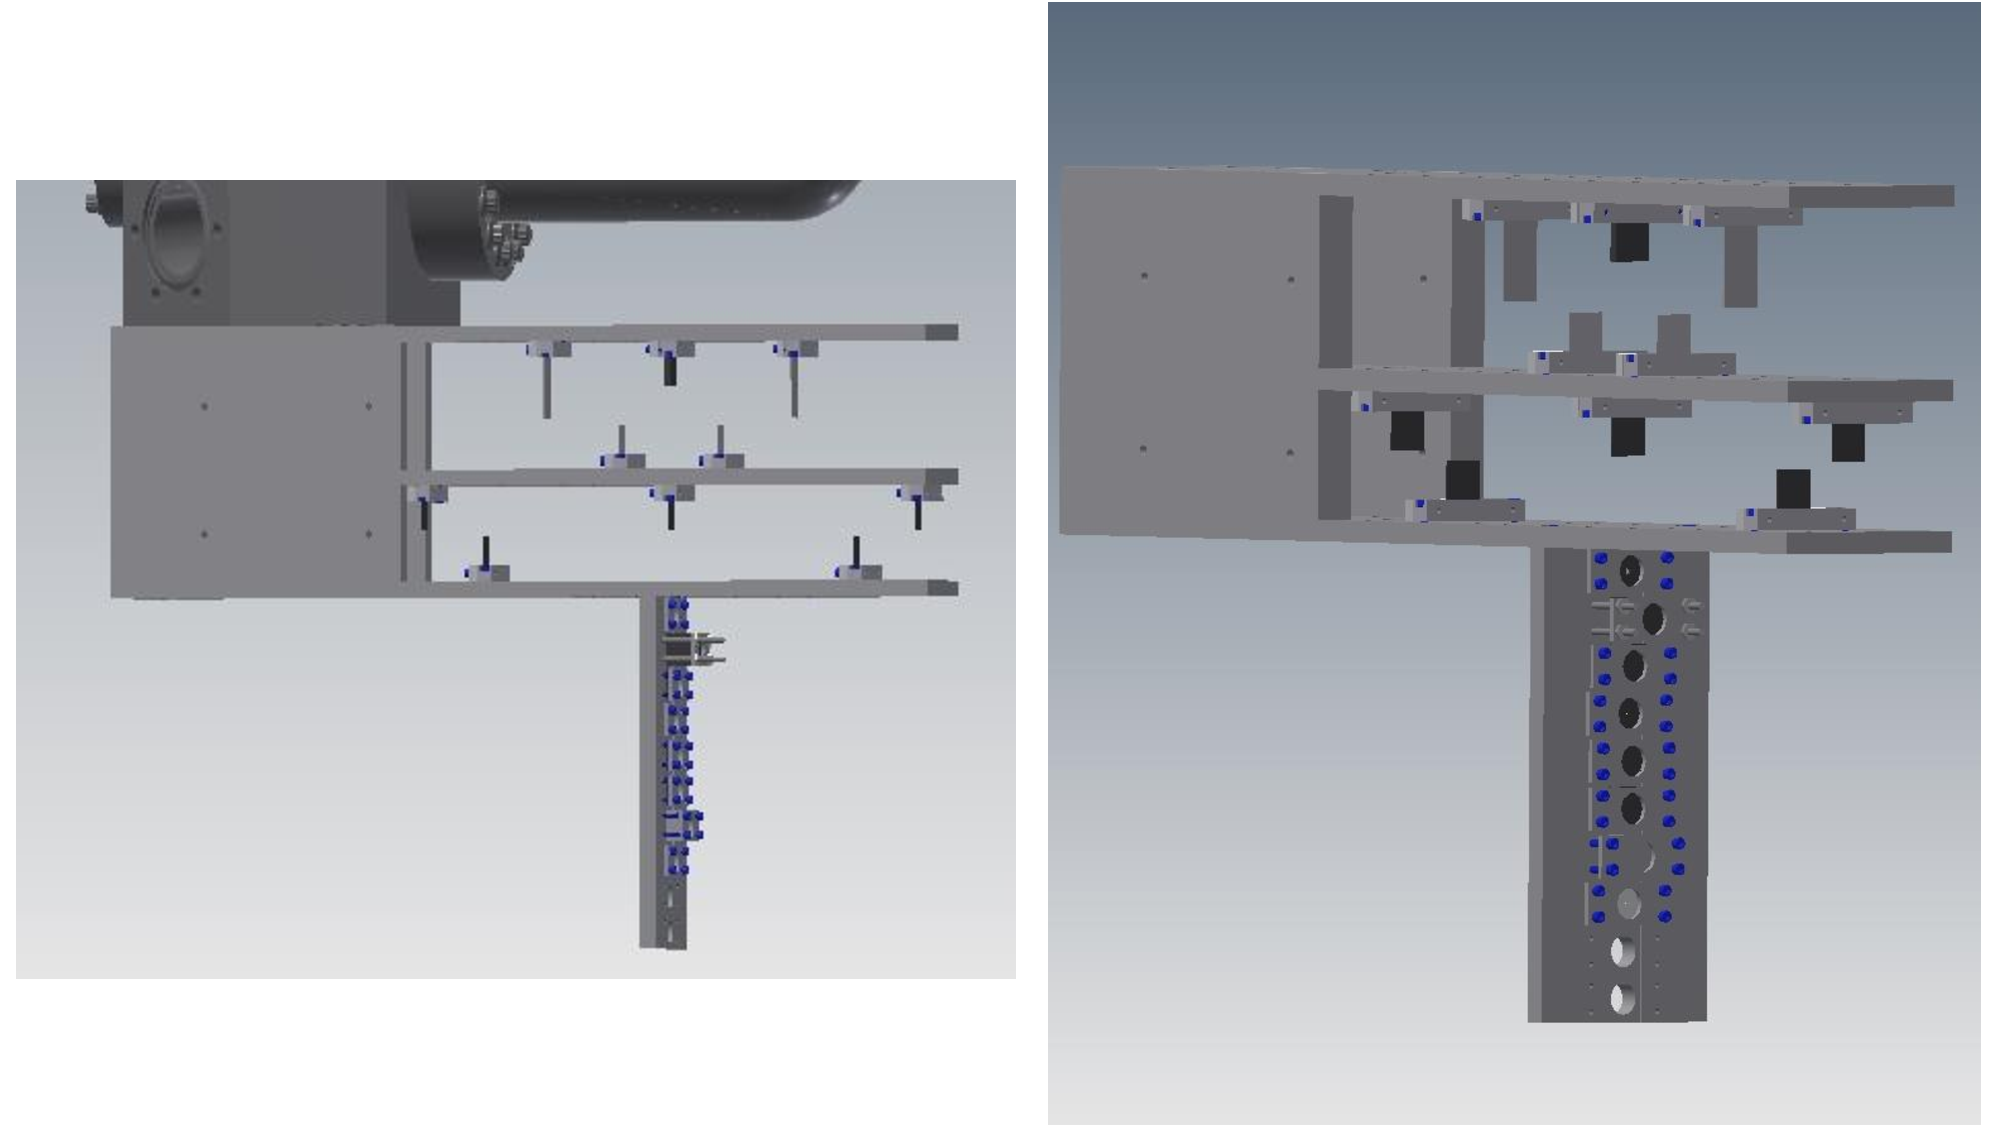
\includegraphics[width =1.0\textwidth]{SolidTgtsCAD.pdf}
\end{center}
%\vspace*{0.5cm}
\caption[tgt-layout]{ CAD views of the solid target ladder. }
\label{fig:SolidTgtsCAD}
\end{figure}

\subsection{Default Targets}
There are several different solid targets  currently in use in the
Hall C Scattering Chamber.  

\begin{itemize}
\item {\bf Optics Target:} This target is an array of carbon foils
  arranged at different Z locations along the beam axis.  Since the
  cryotarget system generally includes a short (typically 4 cm long)
  and a long (typically 15 cm long) cryotarget cell, the usual
  configuration includes foils at $\pm 2$ cm and $\pm 7.5$ cm about
  Z=0 (the spectrometer pivot axis), as well as a target foil at
  Z=0. The resulting picket fence along Z (the beam axis) is useful
  for spectrometer optics calibration.
 

\item {\bf Dummies:} Dummy targets are also provided for subtraction
  of the aluminum cell window background associated with the
  cryotarget windows. The dummy targets are typically sized to provide
  the same radiation length as a full hydrogen cell of the same
  length. The target cell windows are typically each 0.005 $in$ thick,
  and the dummy targets are typically about 1 mm thick. In terms of
  radiation length, 15 cm of LH2 is 1.7\%. Add 2 aluminum cell windows
  each 0.1 mm thick (each 0.11\%) for a total of 1.9\%. Two 1 mm thick
  aluminum dummy targets amount to 2.2\%, a reasonably good match in
  radiation length to the 15 cm target plus its cell windows.

A pair of aluminum dummy targets is provided at a single vertical
target position for each target cell length included in the
cryoloops. For example there will be a dummy target position with
aluminum dummy targets at $\pm 7.5$ cm about Z=0 (the spectrometer
pivot axis and target center) to facilitate subtraction of the
aluminum window background associated with the 15 cm long cryotarget.

\item {\bf Hole Target:} A carbon hole target is also usually provided
  on the solid target ladder at Z=0 to locate the beam. This target
  has a central hole usually 2 mm in diameter. By rastering the beam
  in a pattern at least 2x2 mm$^2$, and using the spectrometer as a
  trigger to detect electrons that miss the hole, an image can be
  constructed from the X \& Y raster magnet currents showing the
  relative location and width of the rastered beam pattern with
  respect to the hole.

\item {\bf Viewer:} A BeO target at Z=0 is also a useful diagnostic to
  check the beam location. The BeO scintillates even at low beam
  current. By viewing the target with a TV camera in the counting
  room, it's easy to see where the beam is.

\item {\bf Carbon:} A general purpose C target capable of handling
  high beam current is also usually on the ladder at Z=0 for other
  assorted diagnostics.

\item {\bf Empty:} An empty target position at Z=0 consists of the
  same frame used to hold the other targets, but without these other
  targets. It's used to see how much beam halo is intercepted by the
  frame.

\item {\bf Home, aka Target Out:} In the ``Home'' target position the
  target motion system is fully retracted to the upper limit
  switch. In this position the beam scoots well underneath the lowest
  target on the solid target ladder. This position is chosen for
  Moller runs and for beam tuning, when the beam position and/or width
  is not well determined.

\item {\bf Other:} Different experiments may require other nuclear
  targets. In the past targets of Li, Be, BeO, C, Al, Ca, Fe, Cu, W,
  Au, Pb, and others have been employed, but not all at once. The
  vertical motion of the target motion system has a limited (24 in)
  range, and solid target choices have to be traded off against the
  number of cryotarget loops (1-3, typically 3), and the number of
  cells per loop (1-2, typically 2).

\end{itemize}

\subsection{Safety Considerations}
Operational restrictions on the maximum beam current and minimum
raster size have to be set in advance for each target by a target
expert on the Hall C staff. The target operator and the staff at MCC
are supposed to look at this page
(\url{http://opweb.acc.jlab.org/internal/ops/ops_webpage/restrictions/ops_restrictions.html})
to insure the targets don't receive more beam current or power density
than they can safely handle.


The main safety issue concerning the non-special targets is that they
will be radioactive (``hot") after they have been exposed to the JLab
beam for an experiment.  Targets may not be removed from the target
chamber or transported from the Hall without concurrence by the
RCG. An SRWP specifies the requirements for target removal and/or
transport. Targets which have been surveyed and released by the RCG
will be stored in the Radiologically Controlled Area (RCA) of the
Target Group in the EEL building.


\subsection{Special Targets}

Some solid targets require special attention. One category will
oxidize when exposed to air, resulting in a large oxygen content in
the target.  Calcium should always be stored in an argon-filled or
evacuated container, or in an oil solution. Calcium can be handled in
air for a limited amount of time (a few hours) if handled with a layer
of oil. The same considerations apply to Lithium.

Other special targets may pose a safety concern, namely ceramic {
  Beryllium-Oxide (BeO)} and { Beryllium (Be)}.  In solid form, BeO is
completely safe under normal conditions of use.  The product can be
safely handled with bare hands.  However, in powder form all Beryllia
is {\bf toxic} when airborne.  { Overexposure to airborne Beryllium
  particulate may cause a serious and sometimes fatal lung disease
  called Chronic Berylliosis. Beryllium has also been listed as a
  potential cancer hazard. Furthermore exposure to Beryllium may
  aggravate medical conditions related to airway systems (such as
  asthma, chronic bronchitis, etc.).}  Since beryllia are mainly
dangerous in powdered form, do not machine, break, or scratch these
products. Machining of the Beryllia can only be performed after
consulting the EH\&S staff.  It is good practice to wash your hands
after handling the ceramic BeO. If handling the pure Beryllium target
or the Beryllium windows, wear gloves and an air filter mask.
Beryllium targets and windows are stored in approved storage locations
(either in Hall C or in the Target RCA) with labels identifying the
contents as Beryllium.

In the past water or helium cooled copper radiators have been used to
generate photons upstream of the physics target. This is not part of
the standard target configuration and therefore not part of this COO.

\subsection{Storage}

The targets are stored in the target group's RCA in the EEL building.
Targets may not be removed from the target chamber or transported from
the hall without concurrence by the RCG.

}
